\documentclass[reprint,amsmath,amssymb,aps,nofootinbib,onecolumn]{revtex4-2}
\usepackage{amsmath,graphicx,latexsym}
\usepackage{braket}
\usepackage{xcolor}

\usepackage[colorlinks=false,bookmarks=false,citecolor=blue,linkcolor=blue,urlcolor=blue]{hyperref}

\renewcommand{\thefigure}{S\arabic{figure}}
\renewcommand{\theequation}{S\arabic{equation}}
%\renewcommand{\thepage}{S\arabic{page}}
\begin{document}

\title{Supplementary Material\\Spin dynamics in single Dy adatoms on graphene/Ir(111)
studied by SP-STM}

\author{A. Curcella}
\affiliation{Institute of Physics, Ecole Polytechnique Fédérale de Lausanne, CH-1015 Lausanne, Switzerland}

\author{D. Sblendorio}
\affiliation{Institute of Physics, Ecole Polytechnique Fédérale de Lausanne, CH-1015 Lausanne, Switzerland}

\author{S. Rusponi}
\affiliation{Institute of Physics, Ecole Polytechnique Fédérale de Lausanne, CH-1015 Lausanne, Switzerland}

\author{M. Pivetta}
\affiliation{Institute of Physics, Ecole Polytechnique Fédérale de Lausanne, CH-1015 Lausanne, Switzerland}

\author{F. Patthey}
\affiliation{Institute of Physics, Ecole Polytechnique Fédérale de Lausanne, CH-1015 Lausanne, Switzerland}

\author{H. Brune}
\affiliation{Institute of Physics, Ecole Polytechnique Fédérale de Lausanne, CH-1015 Lausanne, Switzerland}

\maketitle
\section{Experimental Details}
\subsection{Sample Preparation}
We performed all measurements with a home-built STM \citep{Gaisch1992} operating at 6.5~K (barring the variable temperature measurements) and below \textit{p} $= 10^{-10}$ mbar. A sample preparation chamber sits adjacent to the STM, connected via a UHV transfer stage to allow sample placement into the STM. Before graphene growth, the Ir(111) single crystal is subject to repeated Ar+ sputtering and annealing (1400~K) cycles. A single layer of graphene is grown by chemical vapor deposition (CVD) by exposing the Ir(111) sample to 100 Langmuir of ethylene at 1400~K. The sample is transferred into the STM where Dy atoms are deposited from high purity rods (99.9\%) with an e-beam evaporator at 10~K.
\subsection{Tip Preparation}
We employ antiferromagnetic Mn$_{88}$Ni$_{12}$ tips in all SP-STM measurements. These are produced following the procedures described in Ref. \citep{Forrester2018}, where commercially available 0.25 mm thick Mn$_{88}$Ni$_{12}$ foil is cut into rods, electrochemically etched, then sputtered with Ar+ ions once in an ultra-high vacuum environment before being placed in the STM for use.
\subsection{Telegraph Signal Trace Methodology}
TS traces are taken with the STM feedback loop open, such that the absolute tip-adatom distance remains fixed (neglecting any drift), and initialized in the low conductance state. As pictured in Fig.~2c, the low conductance current typically corresponds to the the current set point before the feedback loop is opened. The adatom is free to switch between the low conductance and high conductance state. The true scattering rate due to the tunneling electrons then, is reflected by the average current of each trace. This average current is calculated for each trace and used as $I_o$ in the model. On the other hand, the $\Delta Z$ pictured in Fig. 2 of the main text is determined by the initial current set point and any thermal drift that occurs during the trace acquisition. We therefore use the average low conductance current $I_{LC}$ in the calculation of $\Delta Z$ (see Sec. \ref{sec:cond-dist}). Tables \ref{table:temp} - \ref{table:curr} contains the average current for each data set used in the main text.  
\begin{table}[h!]
\parbox{.2\linewidth}{}
\hfill
\parbox[b]{.2\linewidth}{
\centering
\begin{tabular}{|c|c|}
 \hline
 T (K) & $I_{avg}$ (pA) 
 \\ [1ex] 
 \hline 
 \hline 
 6.5 & 11.4 \\
 \hline
 6.8 & 12.2 \\
 \hline
 7.3 & 11.8 \\
 \hline
  7.7 & 11.8 \\
 \hline
  8.1 & 12.3 \\
 \hline
  8.5 & 10.8 \\
 \hline
  8.8 & 11.2 \\
 \hline
\end{tabular}
\caption{Average currents in variable temperature dataset.}
\label{table:temp}
}
\hfill
\parbox[b]{.2\linewidth}{
\centering
\begin{tabular}{|c|c|}
 \hline
 $V_{b}$ (mV) & $I_{avg}$ (pA) 
 \\ [1ex] 
 \hline 
 \hline 
 ±1 & 12.4 \\
 \hline
 ±2 & 14.1 \\
 \hline
 ±4 & 16.2 \\
 \hline
 $-$6 & 16.5 \\
 \hline
  ±8 & 17.3 \\
 \hline
\end{tabular}
\caption{Average currents in variable bias dataset.}
}
\label{table:bias}
\hfill
\parbox[b]{.2\linewidth}{
\centering
\begin{tabular}{|c|c|}
 \hline
 $I_{LC}$ (pA) & $I_{avg}$ (pA) 
 \\ [1ex] 
 \hline 
 \hline 
 2.6 & 3.9 \\
 \hline
 5.3 & 7.4 \\
 \hline
 9.1 & 14.1 \\
 \hline
 11.8 & 13.9 \\
 \hline
 24.5 & 28.9 \\
 \hline
 27.6 & 46.9 \\
 \hline
 46.9 & 53.0 \\
 \hline
 58.9 & 93.0 \\
 \hline
 88.9 & 104.1 \\
 \hline
 101.7 & 160.8 \\
 \hline
 179.5 & 217.7 \\
 \hline 
 354.9 & 422.0 \\
 \hline 
 687.2 & 815.8 \\
 \hline
\end{tabular}
\caption{Average currents in variable current dataset.}
\label{table:curr}
}
\hfill
\parbox{.2\linewidth}{}
\end{table}

\section{State Lifetimes}
The lifetimes of the high conductance state $\tau_{HC}$ and low conductance state $\tau_{LC}$ can be simultaneously described by a new quantity, which we define as $\tau^{*}$ \citep{Khajetoorians2013}. The indexes $i,\overline{i}$=LC, HC (with $i\neq \overline{i}$), indicate the low (LC) and high (HC) conductance states. The probability of switching from $ i$ to $\overline{i} $ at time $t$ is given by $ p_{i \overline{i}} $, while the probability of remaining in the same state is given by $ p_{ii} $. We neglect any transient state such that: $ p_{i\overline{i}} + p_{ii} = 1$. The time evolution of $ p_{ii} $ in an infinitesimal time range $dt$ is given by:

\begin{equation}
p_{ii}(t+dt)=p_{i\overline{i}}(t)\frac{dt}{\tau_{\overline{i}}}+p_{ii}(t)\left( 1-\frac{dt}{\tau_i} \right)=(1-p_{ii}(t))\frac{dt}{\tau_{\overline{i}}}+p_{ii}(t)\left( 1-\frac{dt}{\tau_i} \right)=p_{ii}(t)+\frac{dt}{\tau_{\overline{i}}}-p_{ii}(t)\frac{dt}{\tau^*}
\label{eq:prob_dt}
\end{equation}

in which we define $\frac{1}{\tau^*}\equiv\frac{1}{\tau_i}+\frac{1}{\tau_{\overline{i}}}$. Simplifying further from  (\ref{eq:prob_dt}) gives:

\begin{equation}
\frac{dp_{ii}(t)}{dt}=\frac{1}{\tau_{\overline{i}}}-\frac{p_{ii}(t)}{\tau^*}  
\label{eq:diff_p}
\end{equation}

\begin{equation}
p_{ii}(t)=\frac{\tau^*}{\tau_{\overline{i}}}-\exp(-\frac{t}{\tau^{*}})c_1\rightarrow\frac{\tau^{*}}{\tau_{\overline{i}}}-\frac{\tau^{*}}{\tau_i}\exp(-\frac{t}{\tau^*})
\label{eq:sol_diff}
\end{equation}

The condition $p_{ii}(0)=1$ determines the value of the constant $c_1=\frac{\tau^{*}}{\tau_i}$. Note that Eq.~\ref{eq:diff_p} is completely independent of the initial state $i$. Thus, the quantity $\tau^{*}$ governs the time evolution of both LC and HC states. The factors $\frac{\tau^{*}}{\tau_{\overline{i}}} $ and $ \frac{\tau^{*}}{\tau_{i}} $ are the occupancy of the state $\overline{i}$ and $i$, respectively. These quantities are measured experimentally from the telegraph noise signal (TNS) traces.  

\section{Model Hamiltonian}
We use a Hamiltonian of the following form
\begin{equation}
\mathcal{H} = \mathcal{H}_{intra} + \mathcal{H}_{Z} + \mathcal{H}_{CF}  + \mathcal{H}_{ph} + \mathcal{H}_{te}
\end{equation}
The first term describes the intra-atomic exchange between the partially filled \textit{6s}, \textit{5d}, and \textit{4f} shells. This term is the primary novelty of our model and it stems from the recent observation that the external \textit{6s} and \textit{5d} shells are polarized and only partially filled \cite{pivettaMeasuringIntraAtomicExchange2020}. Consequently, the interaction between shells is proportional to the spin component of each shell and can be quantified as:
\begin{equation}
\mathcal{H}_{intra} =\sum_{i\neq j} A_{ij} \, \hat{S}_{i} \cdot \hat{S}_{j} , \qquad i,j = 4f, 5d, 6s
\label{eqSI:H_intra}
\end{equation}
$\hat{S}_{i}$ are the spin operators acting on the shell $i$. Note that for non-polarized external shell (4f model) this term gives a vanishing contribution.
Concerning the 4f5d6s model, the magnitude of the exchange between each shell $A_{ij}$ is taken from DFT calculations \cite{Delin1997,pivettaMeasuringIntraAtomicExchange2020}. These values are scaled according the occupation of each shell, such that they are consistent with the experimental observations of the exchange breaking between the \textit{4f} shell and \textit{5d6s} shells. The second term is the Zeeman term, describing the influence of a stray magnetic field from the STM tip on the Dy adatom. We consider both an axial $B^{tip}_z$ ($z$ parallel to the surface normal $\vec n$) and transverse $B^{tip}_x$ field component, kept as free parameters:
\begin{equation}
\mathcal{H}_{Z} = \mu_{B} B^{tip}_z  \sum_{i} g_{i} \hat{S}_{i,z} + \mu_{B} B^{tip}_x  \sum_{i} g_{i} \hat{S}_{i,x}, \qquad i = 4f, 5d, 6s
\label{eq:zeeman}
\end{equation}
where $g$ is an effective \textit{g}-factor for each shell. In the 4f model, the only non-vanishing contribution is the one acting on the internal \textit{4f} shell. For the 4f5d6s model, we use 1.25, 0.27, and 0.27 for \textit{4f}, \textit{5d}, and \textit{6s} shells \cite{pivettaMeasuringIntraAtomicExchange2020}. The effects of the crystal field are described by the third term. The crystal field only acts on the internal \textit{4f} shell, which has a non-vanishing orbital component. As pointed out in the main text, we assume the orbital moment of the \textit{5d} shell to be quenched due to hybridization with graphene $\pi$-bands \cite{donati2014}. Due to the sixfold symmetry of the adsorption site, $\mathcal{H}_{CF}$ can be expressed as the sum of four Stevens operators $\hat{O}^{n}_{m}$ \cite{baltic2016, Stevens_1952}:
\begin{equation}
\mathcal{H}_{CF} = B^{0}_{2} \hat{O}^{0}_{2} + B^{0}_{4} \hat{O}^{0}_{4} + B^{0}_{6} \hat{O}^{0}_{6} + B^{6}_{6} \hat{O}^{6}_{6}
\label{eqSI:H_CF}
\end{equation}
where the parameters $B^{0}_{2}$, $B^{0}_{4}$, and $B^{0}_{6}$ determines the total zero field splitting and $B^{6}_{6}$ determines the mixing of the magnetic states. The \textit{4f} model values have been taken from Ref.~\cite{baltic2018} while the \textit{4f5d6s} model values are slightly adjusted to take into account the additional spin of the \textit{6s} and \textit{5d} shells. These values are listed in Table~\ref{table:CF}.
\begin{table}[h!]
\centering
 \begin{tabular}{|c||c|c|c|c|}
 \hline
 Model & $B^{0}_{2}$ ($\mu$eV) & $B^{0}_{4}$ (neV) & $B^{0}_{6}$ (neV) & $B^{6}_{6}$ (neV) 
 \\ [1ex] 
 \hline 
 \hline 
 \textit{4f} & -121 & 100 & 1.5 & 0.3 \\
 \hline
  \textit{4f5d6s} & -136 & 17.5 & 2.45 & -5 \\
 \hline
 \end{tabular}
 \caption{CF Parameter Values}
 \label{table:CF}
\end{table}
In both cases, these values are fixed by the size and location of the steps in the XMCD magnetization curves at ±2.7 T and ±5.6 T, which indicate the presence of QTM processes due to level crossings in the energy level diagram. In the \textit{4f} model, the step at +2.7 T is attributed to the crossing between $\ket{7}$ and $\ket{-8}$, mixed due to a small $B^{3}_{6} \hat{O}^{3}_{6}$ term not included in $\mathcal{H}_{CF}$. The step at ±5.6 T is attributed to the crossing between $\ket{7}$ and $\ket{-6}$. Magnetization reversal occurs via QTM through $\ket{\pm 6}$, mediated by electron or phonon scattering in the substrate \cite{baltic2018,baltic2016}. In the \textit{4f5d6s} model, the direct mixing between $\ket{m_7}$ and $\ket{m_{-8}}$ and $\ket{m_7}$ and $\ket{m_{-6}}$ can be explained by considering half of the isotopes of Dy (44$\%$ natural abundance) have nuclear spin $I = 5/2$. The basis $\ket{m_i}=\ket{j_{4f},s_{5d},s_{6s}}$ becomes $\ket{j_{4f},s_{5d},s_{6s},I}$ where $I$ can take on values $-5/2$,$-3/2$, $-1/2$, $+1/2$, $+3/2$, and $+5/2$. The crystal field now mixes the states with $\Delta M_{tot}=\Delta j_{4f} + \Delta s_{5d} + \Delta s_{6s} + \Delta I=6n$, $n\in \mathbb{N}$. Since the multiplicity of $I$ is equal to the symmetry of the crystal field, a level crossing exists between each state $\ket{-8,-0.5,-0.5,I}$ and $\ket{7,0.5,0.5,I^\prime}$ for some $I \ne I^\prime$. The same is true for states $\ket{-6,-0.5,-0.5,I}$ and $\ket{7,0.5,0.5,I^\prime}$ for some $I \ne I^\prime$. The magnitude of $B^{6}_{6}$ is tuned to obtain the same effective level splitting ($10^{-7}$ meV) obtained by applying the Landau-Zener model to the observed magnetization step at +2.7 T \cite{baltic2016, zener1932}. Experimentally, we do not observe any difference between adsorbed Dy adatoms (i.e two species with and without nuclear spin), and therefore conclude that the nuclear spin has no significant influence on the spin dynamics presently studied. \par
We treat the first three terms as the unperturbed Hamiltonian. The fourth term is a perturbation due to spin-phonon coupling that occurs between the Dy adatom and the graphene \cite{Leuenberger2000,cervetti2016}. We utilize a Hamiltonian term of the form:
\begin{equation}
\mathcal{H}_{ph} = \hat{S}^{2}_{4f,-} + \hat{S}^{2}_{4f,+ } + 2 \{\hat{S}_{4f,-},\hat{S}_{4f,z}\} + 2 \{\hat{S}_{4f,+},\hat{S}_{4f,z}\}
\label{eq:ph}
\end{equation}
where $\{ ,\}$ denotes the anticommutator between the two operators, and $\hat{S}_{4f,+}$, $\hat{S}_{4f,-}$ are the spin ladders operators. For both 4f and 4f5d6s model, this term acts only on the internal \textit{4f} shell, the only one carrying a orbital component. $L$ is trivially zero for the 4f model, while it is quenched for the \textit{5d} shell in the 4f5d6s model due to hybridization with graphene bands \cite{donati2014}. The third and fourth term account for first order transitions ($\Delta S = \pm 1$) and the first and second term account for second order transitions ($\Delta S = \pm 2$). The phonon scattering rates associated to a Hamiltonian of this form are discussed further in Section \ref{phonon}. The final term describes the perturbation of the tunneling electrons on the outer \textit{6s} shell. Consistent with previous models \cite{anderson1966,schrieffer1966,appelbaum1967,delgado2010,loth2010,Ternes2015}, we use a Kondo-type Hamiltonian where the tip and substrate electrons are treated as reservoirs:  
\begin{equation}
\mathcal{H}_{te} = \sum_{\alpha,\lambda, \lambda',\sigma,\sigma'} T_{\alpha,\lambda, \lambda'} \frac{\tau^{(\alpha)}_{\sigma\sigma'}}{2} \hat{S}_{6s,\alpha} c^{\dagger}_{\lambda\sigma} c_{\lambda'\sigma'}
\end{equation}
where $\alpha$ can take on values of $x, y, z$ and $0$. $\lambda = (k,\eta)$ defines the single particle state $k$ in the electrode $\eta$ together with the spin $\sigma$ of the transport electrons. $\tau^{(\alpha)}$ and $\hat{S}_{6s,\alpha}$ correspond to the Pauli matrices and spin operators, respectively. In the case of the 4f model, $\hat{S}_{6s,\alpha}$ is replaced by $\hat{S}_{4f,\alpha}$, which means that tunneling electrons interact directly with the internal shell, being the external one non-polarized. For $\alpha = 0$, $\tau^{(0)}$ is defined as the identity matrix, and $T_{o}$ is the Coulomb potential scattering interaction parameter. For $\alpha = x, y,$ and $z$, $T_{\alpha}$ corresponds to the exchange-tunneling interaction parameter between the tunneling electrons and the \textit{6s} (or \textit{4f}) shell of the Dy adatom. In the 4f5d6s model, the exchange coupling that occurs between the \textit{4f} and external \textit{5d} ,\textit{6s} shells enables the reading of the magnetic state of the \textit{4f} shell via a high spin dependent magnetoresistive current \cite{pivettaMeasuringIntraAtomicExchange2020}. \par

\section{Description of scattering rate and tunneling current}

For the description of the electron scattering rates and tunneling current we follow the formalism presented by Delgado \textit{et al.}~\cite{delgado2010}, to which we add the description for substrate phonon scattering \cite{politi_tunneling_1995,cervetti2016} and QTM rates as described in Refs.~\cite{abragam1961,fort1998}. For clarity, we shall give a brief review of this approach to highlight the relevant steps of our implementation in the 4f5d6s model.
The  transitions rates are used to solve a master equation and obtain the diagonal lements of the density matrix $P_M$, expressed in the basis of eigenstates $\ket{M}$ of the unperturbed Hamiltonian ($\mathcal{H_0=\mathcal{Z}}+\mathcal{H}_{ex}+\mathcal{H}_{CF}$).

\subsection{Electron scattering rates}
As mentioned in the text, the value of $\varsigma_T$ (tip-adatom transmission coefficient) is fixed by the experimental value of the elastic current $I_0$ and by the choice of $\varsigma_S$ (substrate-adatom transmission coefficient). From Delgado \textit{et al.}:
\begin{equation}
\varsigma_{T} =  \dfrac{4 \hbar I_0}{2 e \pi \varsigma_{S} \left( \mathcal{F}(V_{b})-\mathcal{F}(-V_{b}) \right)\left( \rho_{S \uparrow} \rho_{T\uparrow} + \rho_{S \downarrow} \rho_{T\downarrow} \right)}
\label{eq:sigmaT}
\end{equation} 

in which $\mathcal{F}$ is the Fermi function. To obtain expression for the electron-induced transition rates in the master equation, we consider the electrodes $\eta$, $\eta^{\prime} \in\lbrace S=surface, T=tip\rbrace$. The electronic rates can be compactly written as:

\begin{equation}
   W_{M,M^{\prime}}^{\eta}=\sum_{\alpha=+,-,z}    \big|\langle M^{\prime}|\hat{S}_{6s,\alpha}|{M}\rangle \big|^2 \mathcal{R}_{\alpha,\eta}
   \label{eq:elec_rates}
\end{equation}
The first term represents the matrix elements and considers the only the scattering wit  the external shell. $\mathcal{R}_{\alpha,\eta}$ is defined as:
\begin{equation}
    \mathcal{R}_{\alpha,\eta}=\dfrac{2\pi}{\hbar}\zeta^2\left( \varsigma_{\eta} \varsigma_{\eta^{\prime}}\mathcal{Q}_{\alpha,\eta \eta^{\prime}} \mathcal{F}_{\eta \eta^{\prime}}(E_{M,M^{\prime}},V_b)+\varsigma_{\eta}^2{Q}_{\alpha,\eta \eta}\mathcal{F}_{\eta \eta}(E_{M,M^{\prime}},0)\right)
    \label{eq:scatt_rates}
\end{equation}
 in which $\zeta$ is the ratio between elastic and inelastic matrix elements, and $\mathcal{F}_{\eta \eta^{\prime}}$ is the Fermi function:
 \begin{equation}
     \mathcal{F}_{\eta \eta^{\prime}}(E_{M,M^{\prime}}-V_b)=\dfrac{E_{M,M^{\prime}}-V_b}{exp[(E_{M,M^{\prime}}-V_b)\beta]-1}
 \end{equation}
 
 and $\mathcal{Q}_{a,\eta \eta^{\prime}}$ describes accounts for the polarization of the electrodes:
 \begin{equation}
     \mathcal{Q}_{+(-),\eta\eta^{\prime}}=\rho_{\eta\downarrow(\uparrow)}\rho_{\eta^{\prime}\uparrow(\downarrow)}, \quad
     \mathcal{Q}_{z,\eta\eta^{\prime}}=\rho_{\eta\uparrow}\rho_{\eta^{\prime}\uparrow}+\rho_{\eta\downarrow}\rho_{\eta^{\prime}\downarrow}
 \end{equation}
 
 Note that the first addend in Eq.~\ref{eq:elec_rates} describes the scattering with electrons originating in one electrode $\eta$ and ending up in the other one $\eta^{\prime}$ ($e_{TS}$ and $e_{ST}$ processes); concerning the second addend, the tunneling electron originates and ends in the same electrode ($e_{TT}$ and $e_{SS}$ processes).
% \section{Description of scattering rates}
% For the description of the electron scattering rates and tunneling current we follow the formalism presented by Delgado \textit{et al.}~\cite{delgado2010}. For clarity, we shall give a brief review of this approach to highlight the relevant steps of our implementation. 

% The STM current can be written as:

% \begin{equation}
% I_{S\rightarrow T} = e \sum_{M,M^{\prime}}P_M(U)\left(W_{M,M^{\prime}}^{S\rightarrow T}-W_{M,M^{\prime}}^{T\rightarrow S}\right)
% \label{eq:stm_curr}
% \end{equation}

% Where $P_M(U)$ are the steady state solutions for each state $M$ of the master equation described below and $W_{M,M^{\prime}}^{\eta \rightarrow \eta'}$ are the scattering rates from state $M$ to $M'$ induced by tunneling electrons that are initially in electrode $\eta$ and end up in electrode $\eta'$.

% The master equation reads:

% \begin{equation}
% \dfrac{dP_M}{dt}=\sum_M P_{M^{\prime}}W_{M^{\prime},M} - P_M\sum_{M^{\prime}}W_{M,M^{\prime}}
% \end{equation}

% $P_M$ are the diagonal elements of the density matrix expressed in the basis of eigenstates $\ket{M}$ of the unperturbed Hamiltonian. In our model, we treat the phonon and tunneling electron Hamiltonian terms as the perturbations. We initialize the master equation by populating the lowest eigenstate $\ket{M}$ at unity ($P_M = 1$). We let the system evolve under the transition rates $W_{M,M^{\prime}}$ (which consider all possible transitions between all electrodes), until steady state solutions for $P_M$ are obtained. This allows for the determination of $\tau^{*}$, $\tau_i$, and $\tau_{\overline{i}}$. 

% \subsection{Electron scattering rates}
% To obtain expression for the electron-induced transition rates in the master equation, we consider the electrodes $\eta$, $\eta^{\prime} \in\lbrace S=surface, T=tip\rbrace$. As is shown in \cite{delgado2010}, a simplified expression for the rates is:

% \begin{equation}
% W_{M,M^{\prime}}^{\eta \eta^{\prime}}=\frac{2 \pi}{\hbar} T_o^2 \nu_T^2 \nu_S^2 \mathcal{F}_{\eta\eta^{\prime}}(E_{M,M^{\prime}} + V_{b})\Upsilon^{\eta\eta^{\prime}}_{M,M^{\prime}}
% \label{eq:elec_rates}
% \end{equation}

% where $T_{o}$ is the Coulomb potential scattering interaction parameter, and $\nu_T$ and $\nu_S$ are proportional to the tip-adatom and adatom-surface hopping integrals. 
% $\Upsilon^{\eta\eta^{\prime}}_{M,M^{\prime}}$ are the rates determined by the terms in the density matrix, and $\mathcal{F}_{\eta\eta^{\prime}}(E_{M,M^{\prime}}\pm V_b )$ is the Fermi-Dirac term to account for the occupation of each state:

% \begin{equation}
% \mathcal{F}_{\eta\eta^{\prime}}(E_{M,M^{\prime}}+ V_{b} )=\dfrac{E_{M,M^{\prime}}+ V_{b}}{exp\left[\left( E_{M,M^{\prime}}+ V_{b}  \right)\beta\right]-1}
% \label{eq:fermi_conv}
% \end{equation}

% in which $E_{M,M^{\prime}}$ is the energy difference between energy levels $\ket{M}$ and $\ket{M^{\prime}}$, $V_{b}$ is the potential difference between electrode $\eta$ and $\eta^{\prime}$, and $\beta=1/k_b T$. The rates $\Upsilon^{\eta\eta^{\prime}}_{M,M^{\prime}}$ of Eq.~\ref{eq:scatt_rates} are explicitly written as:

% \begin{equation}
% \label{eq:ups} 
%     \Upsilon^{\eta\eta^{\prime}}_{M,M^{\prime}}=\dfrac{\delta_{M,M^{\prime}}}{4}\left[  \mathcal{R}^{+}(\eta\eta^{\prime})+ 2\zeta \mathcal{R}^{-}(\eta\eta^{\prime})\langle \hat{S}_{z,\eta\eta^{\prime}} \rangle \right] + \zeta^{2}\left[ \rho_{\eta \downarrow} \rho_{\eta^{\prime}\uparrow} \lvert \hat{S}_{+,\eta\eta^{\prime}}^{M,M^{\prime}}\rvert^{2} + \rho_{\eta \uparrow} \rho_{\eta^{\prime}\downarrow} \lvert {\hat{S}_{-,\eta\eta^{\prime}}^{M,M^{\prime}}}\rvert^{2} +\mathcal{R}^{+}(\eta\eta^{\prime})\lvert \hat{S}_{z,\eta\eta^{\prime}}^{M,M^{\prime}}\rvert^{2} \right]
% \end{equation}

% The terms are separated into elastic and inelastic scattering. Between the first pair of square brackets we find the elastic contributions, as $\delta_{M,M^{\prime}}$ implies. The second square-bracketed terms represent the inelastic contribution.
% The second term of the elastic component describes the magnetoresistive contribution. Note that only the scattering rates between tip and sample, i.e. $\eta\neq\eta^{\prime}$, contribute to the current. However, tip-to-tip and sample-to-sample scattering events, i.e. $\eta=\eta^{\prime}$, contribute to the global rate. $\rho_{\eta}$ is the density of states at Fermi in the electrode $\eta$; $\eta_{\uparrow / \downarrow}$ is the fraction of electrons in the up or down state in electrode $\eta$. The term $\zeta$ is defined as the ratio of the exchange-tunneling interaction parameter $T_{\alpha}$, for $\alpha = x, y,$ and $z$, and the Coulomb potential scattering interaction parameter $T_{o}$. This ratio is proportional to the ratio between inelastic and elastic tunnel matrix elements, and is left as a free parameter within our model. 

% The two terms $\mathcal{R}^{+}$ and $\mathcal{R}^{-}$ are defined as:
% \begin{equation}
%     \mathcal{R}^{\pm}(\eta\eta^{\prime})=\left( \rho_{\eta \uparrow} \rho_{\eta^{\prime}\uparrow} \pm \rho_{\eta \downarrow} \rho_{\eta^{\prime}\downarrow} \right)
%     \label{eq:R_+-}
% \end{equation}

% It is possible to simplify (\ref{eq:scatt_rates}) and (\ref{eq:ups}) to obtain the expression for the inelastic scattering rates used in the main text:

% \begin{equation}
%     W_{MM^{\prime}}^{\eta \eta^{\prime}}=\dfrac{2\pi}{\hbar} \zeta^2 \varsigma_{\eta} \varsigma_{\eta^{\prime}} \mathcal{F}_{\eta\eta^{\prime}}(E_{M,M^{\prime}}+V_{b} )  w_{MM^{\prime}}^{\eta \eta^{\prime}},
%     \label{eq:elec_rates}
% \end{equation}

%  $w_{MM^{\prime}}^{\eta \eta^{\prime}} = \sum_{a} \rho_a \lvert {\textbf{S}_{a,\eta\eta^{\prime}}^{M,M^{\prime}}}\rvert^{2}$ is the inelastic term in Eq. (\ref{eq:ups}) and $\varsigma_{\eta/\eta^{\prime}} = T_o \nu^2_{\eta/\eta^{\prime}}$. Eq. (\ref{eq:ups}) also allows us to obtain expression for the three corresponding contributions to the current by imposing $\eta \neq \eta^{\prime} $.
% The elastic contribution:
% \begin{equation}
% I_0=\dfrac{e}{4} \dfrac{2\pi}{\hbar}  \varsigma_{S} \varsigma_{T} \left( \mathcal{F}_{ST}(V_{ST})-\mathcal{F}_{TS}(V_{TS}) \right) \left( \rho_{S \uparrow} \rho_{T\uparrow} + \rho_{S \downarrow} \rho_{T\downarrow} \right)
% \label{eq:I_0}
% \end{equation}

% The elastic magnetoresistive contribution:
% \begin{equation}
% I_{MR}=\dfrac{e}{4} \dfrac{2\pi}{\hbar}\varsigma_{S} \varsigma_{T}  2 \zeta  \left( \mathcal{F}_{ST}(V_{ST})-\mathcal{F}_{TS}(V_{TS}) \right) \left( \rho_{S \uparrow} \rho_{T\uparrow} - \rho_{S \downarrow} \rho_{T\downarrow} \right) \langle \hat{S}_{z,\eta\eta^{\prime}} \rangle
% \label{eq:I_MR}
% \end{equation}

% And the inelastic contribution:
% \begin{equation}
% I_{in}=\dfrac{e}{4} \dfrac{2\pi}{\hbar}\varsigma_{S} \varsigma_{T} \zeta^2  \left( \mathcal{F}_{ST}(E_{M,M^{\prime}}+V_{ST})-\mathcal{F}_{TS}(E_{M,M^{\prime}}+V_{TS}) \right) \sum_{a} \rho_a \lvert {\hat{S}_{a,\eta\eta^{\prime}}^{M,M^{\prime}}}\rvert^{2}
% \label{eq:I_in}
% \end{equation}

% Since the elastic contribution is orders of magnitude larger than the inelastic contribution, we take the average tunneling current $I_{avg}$ as equal to $I_{o}$. Treating $\zeta$ and $\varsigma_{S}$ as free parameters, and choosing reasonable values for $\rho_T$, allows us to solve for $\varsigma_{T}$ for the experimentally-known tunneling bias and current:

% \begin{equation}
% \varsigma_{T} =  \dfrac{4 \hbar I_0}{2 e \pi \varsigma_{S} \left( \mathcal{F}_{ST}(V_{ST})-\mathcal{F}_{TS}(V_{TS}) \right)\left( \rho_{S \uparrow} \rho_{T\uparrow} + \rho_{S \downarrow} \rho_{T\downarrow} \right)}
% \label{eq:sigmaT}
% \end{equation} 
% This is advantageous as we expect $\varsigma_{T}$ to depend on the tip-adatom distance defined by the tunneling conditions, while $\zeta$ and $\varsigma_{S}$ are fixed.  

\subsection{Phonon scattering rates}
\label{phonon}
In addition to electron scattering, we also consider phonon absorption and relaxation between the graphene and Dy adatom. We assume a 2D phononic bath similar to Ref. \cite{cervetti2016}. The 2D rates are functions of the 2D mass density of graphene $\rho_{gr}$, the speed of sound in graphene $c$, and the Bose-Einstein distribution. These rates are similar to the corresponding 3D rates defined by Eq.~10 in Ref. \cite{politi_tunneling_1995}, modified accordingly \cite{cervetti2016}: 

\begin{equation}
    W_{MM^{\prime}}^{ph} =
    \begin{cases}
        \displaystyle
        \frac{ \nu_{ph}}{\rho_{gr} c^4 \hbar^3} \frac{E_{M,M^{\prime}}^2}{exp(\beta E_{M,M^{\prime}}) - 1} w_{4f,MM^{\prime}}\\
        \\
        \displaystyle
         \frac{ \nu_{ph}}{\rho_{gr} c^4 \hbar^3} \left( 1 + \frac{E_{M,M^{\prime}}^2}{exp(\beta E_{M,M^{\prime}}) - 1}\right) w_{4f,MM^{\prime}}
    \end{cases}
\label{eq:phonon_rates}    
\end{equation}

% \begin{equation}
%  W_{MM^{\prime}}^{ph} =  \frac{ \nu_{ph}}{\rho_{gr} c^4 \hbar^3} \frac{E_{M,M^{\prime}}^2}{e^{\beta E_{M,M^{\prime}}} - 1} w_{MM^{\prime}}
%  \label{eq:phabs}
% \end{equation}

% \begin{equation}
%  W_{MM^{\prime}}^{ph} =  \frac{ \nu_{ph}}{\rho_{gr} c^4 \hbar^3} \left( 1 + \frac{E_{M,M^{\prime}}^2}{e^{\beta E_{M,M^{\prime}}} - 1}\right) w_{MM^{\prime}}
%  \label{eq:phrel}
% \end{equation}
\noindent
for phonon adsorption and relaxatio, respectively. In eq.~\ref{eq:phonon_rates}, $\rho_{gr} = 7.7 \times 10^{-7}$ kg/m$^2$ and $c = 2.1 \times 10^4$ m/s \cite{Falkovsky2007}. $w_{4f,MM^{\prime}}$ are the phonon matrix elements squared (acting only on the \textit{4f} shell) and $\beta = 1/ k_{b} T$. We also include $\nu_{ph}$ to account for the spin-phonon coupling between the 2D graphene and Dy adatom and any other proportionality factors not explicitly mentioned in Eq.~\ref{eq:phonon_rates} (see Refs. \cite{Leuenberger2000,cervetti2016}). Note that $\nu_{ph}$ is different for transitions with $\Delta m = \pm 1$ and $\Delta m = \pm 2$. The difference is negligible in the context of the model results presented here, thus we keep it constant for all transitions and all tunneling conditions. A value of $\nu_{ph} = 6 \times 10^{-4}$ is used. \par

\subsection{QTM rates}
We use the expression for QTM rates in and out of resonance derived in Ref. \cite{abragam1961,fort1998}. The tunneling rate is given by:
\begin{equation}
W^{QTM}_{M,-M} =  \frac{2 \tau^{*}_{M} \omega^{2}_{o}}{1 + (\tau^{*}_{M} \omega_{1})^2}
\label{eq:qtm}
\end{equation}
where $\tau^{*}_{M}$ is the characteristic lifetime of state $M$ in the absence of QTM, $\omega_{o} = \Delta E_{M,-M}/\hbar$ in resonance and $\omega_{1} = \Delta E_{M,-M}/\hbar$ out of resonance. 

\subsection{Master equation}

The rates in Eqs.~\ref{eq:elec_rates},~\ref{eq:phonon_rates}, and~\ref{eq:qtm}, are used in a master equation to obtain the diagonal elements of the density matrix, $P_M$:
\begin{equation}
    \dfrac{dP_M}{dt}=\sum_M P_{M^{\prime}}W^{el-ph}_{M^{\prime}M} - P_M\sum_{M^{\prime}}W^{el-ph}_{MM^{\prime}}+W^{QTM}_{M,-M}(P_{-M}- P_{M})
    \label{eq:master}
\end{equation}
in which $W^{el-ph}_{M^{\prime}M}$ are the total electron-phonon transition rates:
\begin{equation}
    W^{el-ph}_{M^{\prime}M}=W^{T}_{M^{\prime}M}+W^{S}_{M^{\prime}M}+W^{ph}_{M^{\prime}M}
\end{equation}

The populations derived in Eq.~\ref{eq:master} can then be used to estimate the inelastic component of the tunneling current and the magnetoresistive term \cite{delgado2010}:
\begin{gather}
    I_{in}=\text{e}\sum_M \Tilde{P}_M \sum_{M^{\prime}} (W^{T}_{MM^{\prime}}-W^{S}_{M^{\prime}M})\sum_M \Tilde{P}_M\\
    %I_{MR}&=\text{e}\dfrac{2\pi}{4\hbar}\varsigma_S\varsigma_T (\mathcal{F}_{TS}(E_{M,M^{\prime}}-V_b)-\mathcal{F}_{ST}(E_{M,M^{\prime}}+V_b))2\zeta (\rho_{T\uparrow}\rho_{S\uparrow}-\rho_{T\downarrow}\rho_{S\downarrow})\sum_M P_M \langle M|\hat{S}_{6s,z}|{M}\rangle
    I_{MR}=I_0\zeta\dfrac{\rho_{T\uparrow}-\rho_{T\downarrow}}{\rho_{T\uparrow}+\rho_{T\downarrow}}\sum_M \tilde{P}_M\langle M|\hat{S}_{6s,z}|{M}\rangle
    \label{eq:I_MR}
\end{gather}
in which $\tilde{P}_M$ represents the equilibrium population of the state $\ket{M}$. Note that the dependency of $I_{MR}$ upon $\varsigma_S$ and $\varsigma_T$ is included inside $I_0$.

\subsection{4f model}
The previous description is valid also in the case of the 4f model, provided we replace the $\hat{S}_{6s,\alpha}$ with $\hat{S}_{4f,\alpha}$, \textit{i.e.} the electrons scatter directly with the internal \textit{4f} shell. This of course changes the value of the matrix elements involving the spin operators. This changes the values of 




\section{Conductance Distance Measurements and Tip Field}
\label{sec:cond-dist}
\begin{figure*}[ht!]
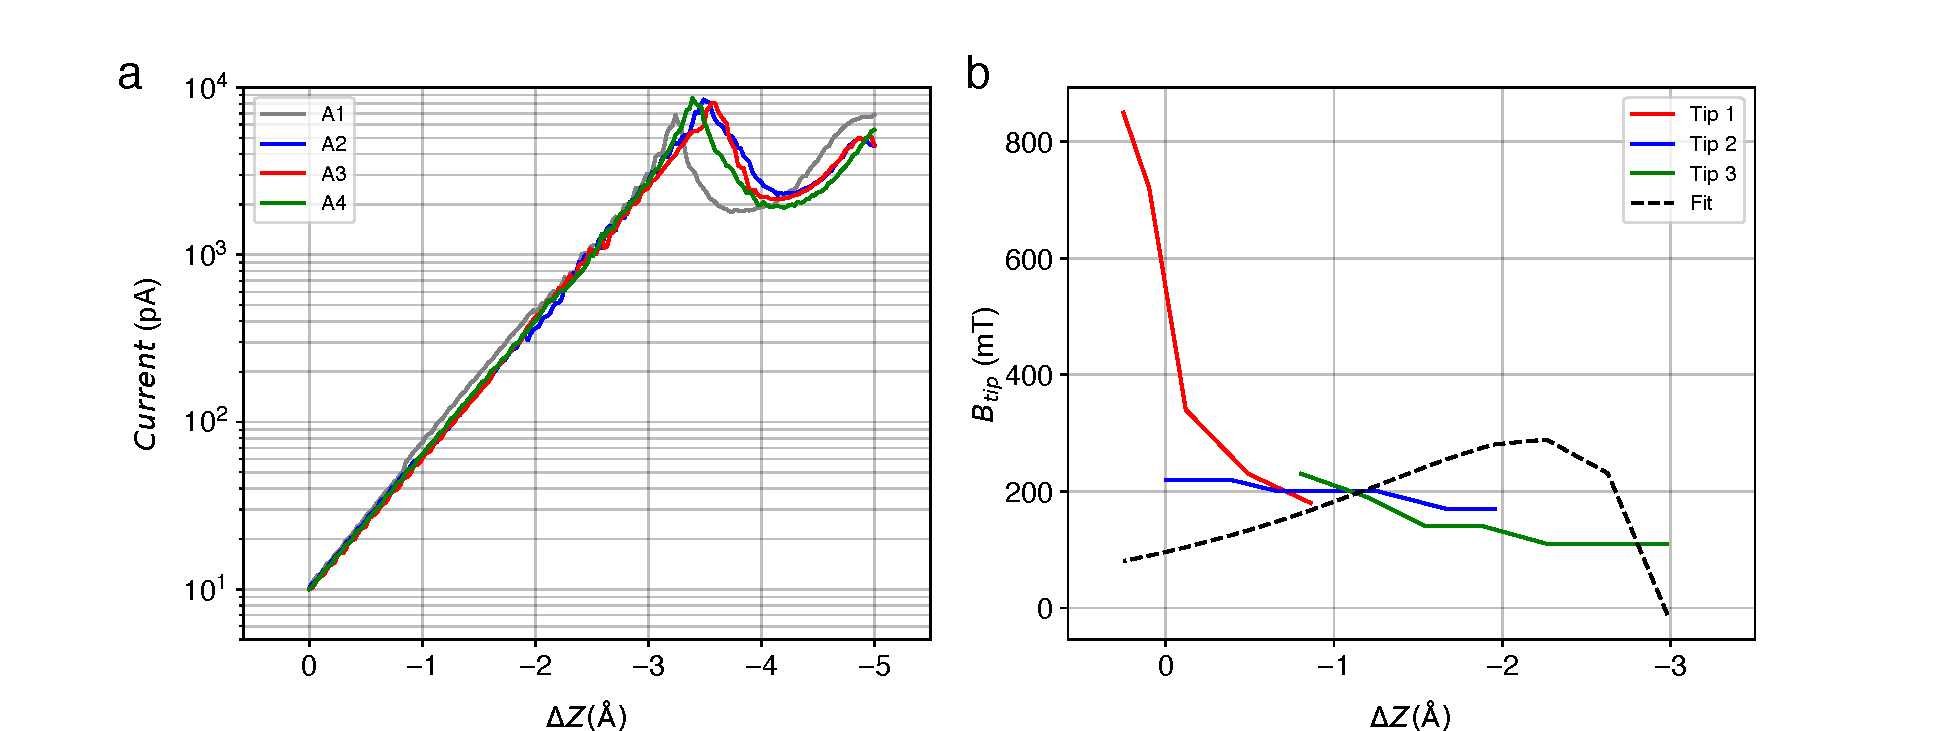
\includegraphics[width=0.98\textwidth]{fields_fit2.pdf}
\caption{Conductance Distance Measurements and Tip Field. (\textbf{a}) Conductance distance measurements over 4 different Dy adatoms ($V_{b} = +2$ mV,$I_o = 10$ pA, $T = 6.5$ K). (\textbf{b}) Tip field $B^{tip}$ values used in the polarized model to fit the experimental data. The simple fit (dashed) of Eq. \ref{eq:fit} is included for comparison. 
\label{fig:fields} }
\end{figure*}

As the tip field $B^{tip}$ is unknown, we choose the value that best fits the experimental data. The Zeeman term in the Hamiltonian (Eq. \ref{eq:zeeman}) contains both an axial component $B^{tip}_z$ and transverse component $B^{tip}_x$ acting on each shell. The transverse component $B^{tip}_x$ has a negligible effect on the occupancy and the characteristic lifetime $\tau^{*}$; we therefore limit our discussion to the axial component such that $B^{tip} = B^{tip}_z$. 
To better understand the distance dependence of $B^{tip}$, we performed conductance-distance measurements above the Dy adatoms. Fig.~\ref{fig:fields}a shows the results of these measurements over 4 different adatoms (A1-A4). A clear departure from the exponential behavior expected from electron tunneling occurs for $\Delta Z < -3$ \text{\normalfont\AA}. An exponential fit ($I(\Delta Z) = I_o e^{-\kappa \Delta Z}$) of the region $\Delta Z > -3$ \text{\normalfont\AA} reveals a decay constant $\kappa$ of 1.9. The decay constant allows us to map the low conductance current and bias ($I_{LC}$ and $V_{b}$) of each TNS trace in the variable bias (Tip 1 in Fig.~\ref{fig:fields}b) and variable current datasets (Tips 2 and 3 in Fig.~\ref{fig:fields}b) onto $\Delta Z$. 

Fig.~\ref{fig:fields}b shows the $B^{tip}$ needed to fit the experimental datasets as a function of $\Delta Z$. In the variable temperature dataset, we assume a constant field $B^{tip}$ = 430 mT for all temperatures. If we assume the tip field $B^{tip}$ is composed of a dipolar component and an exchange component of the form:
\begin{equation}
B^{tip}(\Delta Z) =  \frac{B^{dip}_{o} Z^{3}_{o}}{(Z_{o}+\Delta Z)^{3}} + B^{exch}_{o} e^{-\Delta Z/d}
\label{eq:fit}
\end{equation}
where $Z_o$ is the relative tip-adatom distance and $d$ is the exchange decay constant, and $B^{exch}_{o}$ and $B^{dip}_{o}$ are the magnitudes of the magnetic field at $Z_o$. A fit of $B^{tip}$ as a function of $\Delta Z$ can be made by restricting values for $Z_o$, $B_{dip}$, $B_{exch}$, and $d$. The fit in Fig.~\ref{fig:fields}b uses the following values: $Z_o = 4.8$ \text{\normalfont\AA}, $B^{dip}_o = -60$ mT, $B^{exch}_o = 154$ mT, and $d = 1.5$ \text{\normalfont\AA}. Different goodness-of-fit can be achieved by changing these parameters. However, the difference in trends between this simple fit and the tip field $B^{tip}$ needed suggests a more complicated scaling. As nanoscale changes in the tip apex can change from measurement to measurement, we expect the tip field felt by the Dy adatom to change as well. Each tip in Fig.~\ref{fig:fields}b) consists of a single continuously acquired dataset where no observed changes in tip behavior occurred. While the fit assumes a simple dipolar and exchange scaling, the true tip field may have more complex scaling determined my the local tip geometry.

\section{Variable Bias and Variable Current Results for the \textit{4f} Model}
\begin{figure*}[h!]
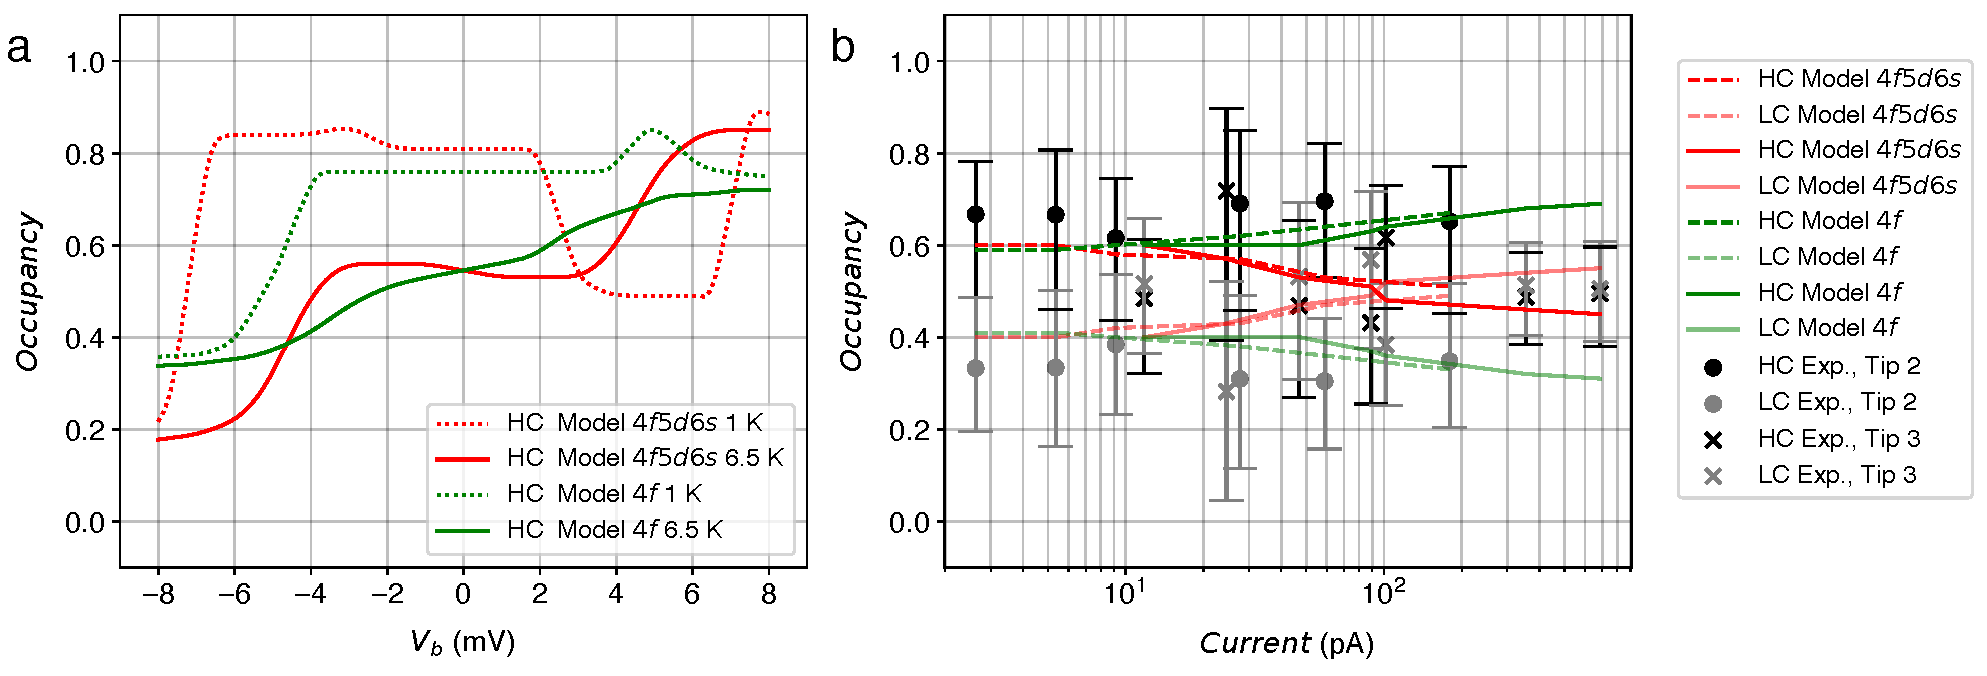
\includegraphics[width=0.5\textwidth]{model_4f.pdf}
\caption{\textit{4f} Model Variable Bias. \textit{4f} (green) and \textit{4f5d6s} (red) model predictions of state occupancy as a function of bias at 1 K (dashed) and 6.5K (solid) for $\rho_{T \uparrow}$ = 0.7. Note that for simplicity, the tip field $B_{tip}$ (100 mT) and $I_o$ (15 pA) is kept constant for each bias. 
\label{fig:bias_curr} }
\end{figure*}

At 6.5 K, there is an inappreciable difference between the \textit{4f} and \textit{4f5d6s} model in the state occupancy and lifetimes in the variable bias dataset (Fig. 4a-b of main text) due to the temperature smearing of the transition pathways. In both cases, a set of free parameters exists that agrees with the experimental data reasonably well. However, if considering the occupancy at 1 K rather than 6.5 K the difference becomes more apparent. Fig.~\ref{fig:bias_curr}a compares the two models at 1 K and 6.5 K. At 1 K, the presence of the single transition pathway available in the \textit{4f} model is visible at at $|V_b|>5.5$ meV, while at $|V_b|<5.5$ meV, the asymmetry is primarily determined by the tip field $B^{tip}$. At higher temperature, the delineation between these two regimes is both spread across several meV and smoothed.   


\bibliographystyle{naturemag}
\bibliography{bib.bib}

\end{document}



















